\begin{appendices}
    \section{Code for the AMSIMP Global Forecast Model}\label{model_code}
    \begin{minted}[mathescape,linenos,frame=lines]{python}
def model(epochs, bs):
    # Number of elements.
    n = len(os.listdir("processed_dataset/"))
    lst_n = np.linspace(1, n, n)
    
    # Define training dataset and validation dataset.
    # Training.
    train_ns = lst_n[:int(0.7 * n)]
    train_generator = DataGenerator(
        train_ns,
        batch_size=bs,
    )
    print("Training dataset created.")
    
    # Validation.
    val_ns = lst_n[int(0.7 * n):int(0.9 * n)]
    val_generator = DataGenerator(
        val_ns, 
        batch_size=bs,
        shuffle=False
    )
    print("Validation dataset created.")
    
    with mirrored_strategy.scope():
        # Create, and train models.
        # Optimiser.
        opt = Adam(lr=1e-3, decay=1e-5)
        # Create model.
        model = Sequential()

        # First layer.
        model.add(
            ConvLSTM2D(
                filters=64, 
                kernel_size=(7, 7),
                input_shape=(6, 179, 360, 3), 
                padding='same', 
                return_sequences=True, 
                activation='tanh', 
                recurrent_activation='hard_sigmoid',
                kernel_initializer='glorot_uniform', 
                unit_forget_bias=True, 
                dropout=0.3, 
                recurrent_dropout=0.3, 
                go_backwards=True
            )
        )
        # Batch normalisation.
        model.add(BatchNormalization())
        # Dropout.
        model.add(Dropout(0.1))
        
        # Second layer.
        model.add(
            ConvLSTM2D(
                filters=32, 
                kernel_size=(7, 7), 
                padding='same', 
                return_sequences=True, 
                activation='tanh', 
                recurrent_activation='hard_sigmoid', 
                kernel_initializer='glorot_uniform', 
                unit_forget_bias=True, 
                dropout=0.4, 
                recurrent_dropout=0.3, 
                go_backwards=True
            )
        )
        # Batch normalisation.
        model.add(BatchNormalization())
        
        # Third layer.
        model.add(
            ConvLSTM2D(
                filters=32, 
                kernel_size=(7, 7), 
                padding='same', 
                return_sequences=True, 
                activation='tanh', 
                recurrent_activation='hard_sigmoid', 
                kernel_initializer='glorot_uniform', 
                unit_forget_bias=True, 
                dropout=0.4, 
                recurrent_dropout=0.3, 
                go_backwards=True
            )
        )
        # Batch normalisation.
        model.add(BatchNormalization())
        # Dropout.
        model.add(Dropout(0.1))

        # Final layer.
        model.add(
            ConvLSTM2D(
                filters=32, 
                kernel_size=(7, 7), 
                padding='same', 
                return_sequences=True, 
                activation='tanh', 
                recurrent_activation='hard_sigmoid', 
                kernel_initializer='glorot_uniform', 
                unit_forget_bias=True, 
                dropout=0.5, 
                recurrent_dropout=0.3, 
                go_backwards=True
            )
        )
        # Batch normalisation.
        model.add(BatchNormalization())

        # Add dense layer.
        model.add(Dense(3))
    
    # Compile model.
    model.compile(
        optimizer=opt, 
        loss='mse'
    )
    # Summary of model.
    model.summary()

    # Train.
    model.fit(
        train_generator,
        validation_data=val_generator,
        epochs=epochs,
        callbacks=[
            tf.keras.callbacks.EarlyStopping(
                monitor="val_loss", min_delta=0, patience=2, mode="auto"
            )
        ],
    )
    
    return model
    \end{minted}
    
    \section{Comparison against Previous Model}\label{old_model}
    \begin{figure}[H]
        \centering
        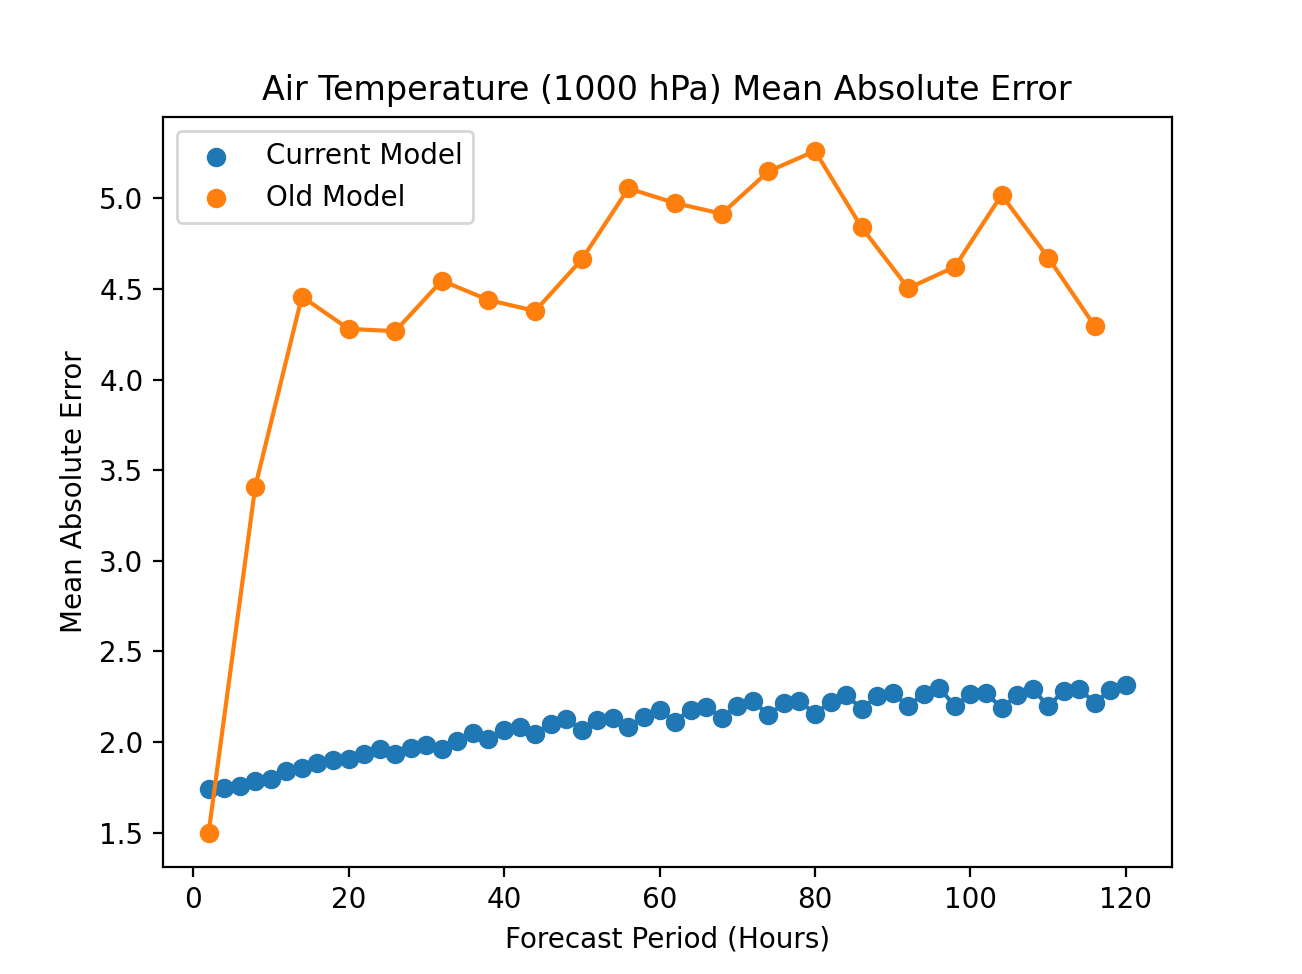
\includegraphics[width=.7\linewidth]{Plots/Results/Temperature/t1000_mae.png}
        \caption{MAE for Air Temperature at 1000 hPa}
    \end{figure}
    
    \begin{figure}[H]
        \centering
        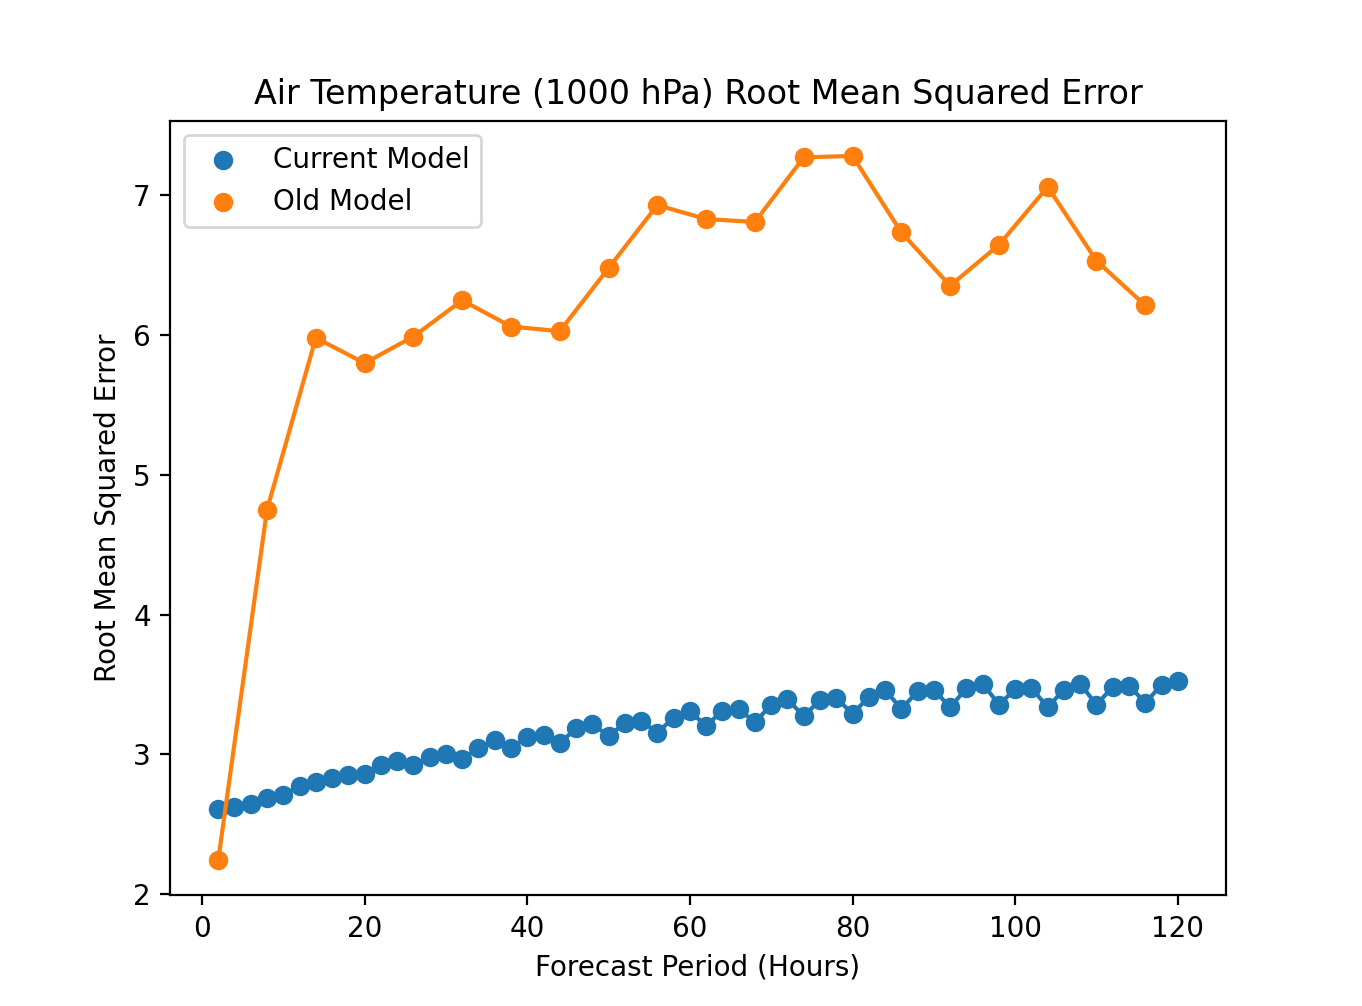
\includegraphics[width=.7\linewidth]{Plots/Results/Temperature/t1000_rmse.png}
        \caption{RMSE for Air Temperature at 1000 hPa}
    \end{figure}
\end{appendices}